\documentclass[11pt]{article}

\usepackage{graphicx}
\usepackage[utf8]{inputenc}
\usepackage{amsmath}
\usepackage[top=1in, bottom=1.25in, left=1.25cm, right=1.25in]{geometry}


\begin{document}

\begin{minipage}{0.33\textwidth}

\underline{\textbf{Grundformeln:}}\\
WS: $R = \frac{U}{I} = \frac{\rho \cdot l}{A}$; $[R] = 1\frac{V}{A} =1 \Omega$\\
Leitwert: $G = \frac{1}{R}$\\
Maschensatz: $\sum U_i = 0$\\
Knotensatz: $\sum I_i = 0$\\
Reihe WS: $R_{ges} = \sum R_i$\\
Parallel WS: $\frac{1}{R_{ges}} = \sum \frac{1}{R_i}$\\
\phantom{ss} Spezialfall: $R_{ges} = \frac{R_1 \cdot R_2}{R1+R2} $\\
Spannungs-Teiler: $\frac{U_1}{U_2} = \frac{R_1}{R_2}$\\
Strom-Teiler: $\frac{I_1}{I_2} = \frac{R_2}{R_1}$\\
Leistung: $P =U \cdot I = \frac{U^2}{R} = I^2 \cdot R $ \\
\phantom{ssssssssss} $[P] = 1V \cdot A =1 W$\\
Kein Strom $\Rightarrow$ U in Masche gleich!\\

\underline{\textbf{Kondensator:}}\\
Kapazität: $C = \frac{Q}{U} = \frac{\varepsilon \cdot A }{d},$\\
\phantom{ssssssssssii} $[C]=1F$\\
\phantom{sssssssssssii} $d =$ Plattenabstand\\
Ladung: $q = \int_{t_0}^t i(\tau) d\tau + q_0$\\
\phantom{sssssssis} $\stackrel{homogen}{=} I \cdot t$\\
\phantom{ssssssssssii} $[q]=1C$\\
Spannung: $U = \frac{Q}{C}$\\
\phantom{ssi} $= \frac{1}{C} \cdot (\int_{t_0}^t i(\tau) d\tau + q_0)$\\
Kond. parallel: $C_{ges} = C_1 + C_2$\\
Kond. in Reihe: $C_{ges} = C_1 || C_2$\\
Kond. in Reihe: $Q_1 = Q_2 = Q_{12}$\\

$U_a(t) = k_1 + k_2 \cdot e^{-\frac{t-t_0}{\tau}}$\\
Berechne $k_1$ durch $t \rightarrow \infty$, oft $U_B$\\
$k_2$ durch $t = 0$, oft $-U_B$\\
$[k] = 1V$\\

$\tau = R \cdot C; [\tau] = 1s$\\
\phantom{ss}falls WS in Reihe $\Rightarrow$ parallel\\
$t =\frac{T}{2} = \frac{1}{2f}$\\
Zeit Auf-/Entlanden: $t = 3\tau$\\

"eingeschwungen" $\Rightarrow i_C = 0$\\

Arbeit(=Energie): $W = \int_0^\infty P dt$\\
\phantom{sssssssss} $= \frac{U_b^2 \cdot C}{2} $\\
\phantom{sssssssss} $= [W] = 1J $\\
$W_{Zyklus} = W_a + W_e$\\

$\overline{P} = \frac{W_{Zyklus}}{T}$\\

Tiefpass: Oben R, Mitte C, Integrator
\end{minipage}%
~~~~~~~
\begin{minipage}{0.33\textwidth}
%\vspace{-11.5 cm}

\underline{\textbf{Felder:}}\\
Stromdichte: $S=\frac{I}{A}$\\
Feldstärke: $E=\frac{S}{\kappa}$\\
Spannungsabfall: $U=E \cdot l$\\
Pot.: $\varphi (x)= \int_x^0 E(s)ds + \varphi(0)$\\
Stromstärke: $I = \oint H ds = H \cdot 2\pi r$\\
Mag.Feldstr.: $H = \frac{I}{2\pi d}, [H] = 1\frac{A}{m}$\\
Kraft pro Leitungslänge:\\
\phantom{ss} $F=Q \cdot v \cdot B, [F] = 1N$\\
Ladung pro mm: $Q = \rho \cdot V$\\
$e^-$, Drift-Gesch.: $v = \frac{S}{\rho}, [v] = 1\frac{m}{s}$\\
Flussdichte: $B=\mu \cdot H, [B] = 1 \frac{Vs}{m^2}$\\
 
 \underline{\textbf{(Koaxial-)Leitungen}}:\\
$R_W = \sqrt{\frac{L'}{C'}}$\\
    \phantom{sssi} $=\frac{\sqrt{\epsilon_R \cdot \mu_R}}{c_0 \cdot C'}$\\
    \phantom{sssi} $=\frac{\sqrt{\mu_R} \cdot ln(\frac{d_a}{d_i})}{2c_0 \cdot \pi \cdot \epsilon_0 \cdot \sqrt{\epsilon_R}}$\\
% Gleichung C', L'
$C = \frac{1}{\sqrt{L' \cdot C'}} = \frac{c_0}{\sqrt{\epsilon_r \cdot \mu_s}}$\\
$C' = \frac{2\pi \epsilon_0 \epsilon_r \cdot s}{ln(\frac{d_a}{d_i})}$\\
$L' = \frac{\sqrt{\epsilon_r \mu_r}}{c_0 \cdot \sqrt{C'}}$\\
$X' = \frac{X}{l}$\\

$k_0 = \frac{R_w}{R_w + R_i} $\\
$r_a = \frac{R_a - R_w}{R_a + R_w} $\\
$k_a = 1 + r_a = k_1$\\
$R_w ==$ WS der Leitung\\
$R_i ==$ WS vor der Leitung\\
$R_a ==$ WS nach der Leitung\\
Reflexion: $U_r(l,t) = r_a \cdot U_k(l,t)$\\
Anfang: $U_k(0,t)=k_0 \cdot U_{q}(t)$\\
Ende: $U_k(x,t)= k_0 \cdot U_{q}(t-\Delta t)$\\
$\Delta t = \frac{l}{c} = \frac{l}{\lambda f}$\\
Auskoppeln Gatter:\\
\phantom{ss} $U_1(t) = k_a \cdot U_1(x,t)$\\
V Ende Leitung: $u_a = k_0 \cdot k_a \cdot u_q$\\

LW-Leitung: $\alpha = \frac{L_P}{l}; [\alpha] = 1 \frac{dB}{m}$\\
Lichtleistung: $L_P = 10 \cdot lg\frac{P_e}{P_a} dB$\\
\phantom{sssssississsssss} $L_P = l \cdot \alpha$\\
\phantom{sssssississsssss}$ [L_P] = 1dB$\\



\end{minipage}%
~~~~~~
\begin{minipage}{0.33\textwidth}
\underline{\textbf{Operationsverstärker:}}\\
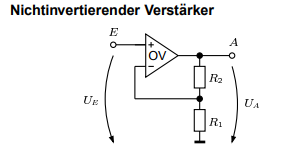
\includegraphics[scale=0.40]{NIOV.png}
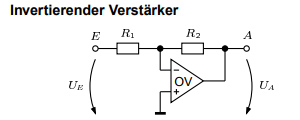
\includegraphics[scale=0.40]{IOV.png}
$U_D = 0 \Rightarrow I_N = 0, U_N = 0$\\

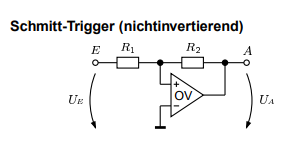
\includegraphics[scale=0.40]{NISTOV.png}\\
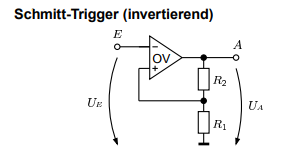
\includegraphics[scale=0.40]{ISTOV.png}\\
Umschalten, wenn $U_D = 0$\\
$U_A \in \{U_B,0\}$\\
$U_D = 0 = U_P - U_{E_{HL}}$\\
\phantom{sssi}$\Rightarrow U_{E_{HL}} = \frac{U_{A_{max}} \cdot R_2}{R_1 + R_2}$\\
$U_D = 0 = U_P - U_{E_{LH}}$\\
\phantom{sssi}$\Rightarrow U_{E_{LH}}= \frac{ U_{A_{min}} \cdot R_2}{R_1 + R_2}$\\
Diode: $\Rightarrow U_{E_{LH}} = 0$\\
Schalthysterese:\\
\phantom{sssssi} $H = |U_{E_{HL}} - U_{E_{LH}}|$\\

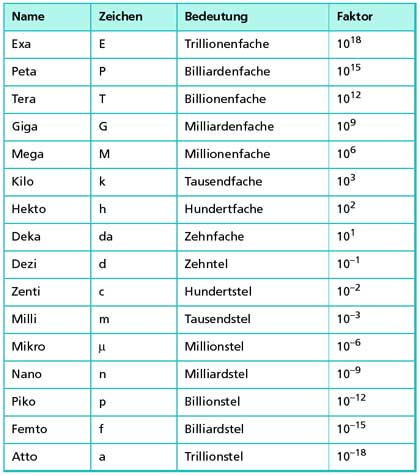
\includegraphics[scale=0.40]{Zehnerpotenzen.jpg}

\end{minipage}%

\newpage

\begin{minipage}{0.33\textwidth}

\underline{\textbf{Diode:}}\\
Gesperrt: $U_D < U_{F_0}$\\
Leitend: $\Rightarrow U_D = U_{F_0}$\\
Reale Diode sperrt: $\Rightarrow I_D = -I_S$\\

\underline{\textbf{Transistor:}}\\
$I_G \stackrel{!}{=} 0A$\\

n-Kanal:\\
- Pfeil auf Gate\\
- Sperrt: $U_{GS} < U_{th}$\\
- Leitet: $\Rightarrow U_{DS} \geq 0$\\
\phantom{sssssiisssi}$\Rightarrow I_D \geq 0$\\

\[I_{D_N} = \left\{
  \begin{array}{lr}
    0 & , U_{GS} < U_{th}~Sperrbereich\\
    \frac{1}{2} \cdot \beta \cdot(U_{GS} - U_{th})^2  \ & , U_{DS} \ge U_{GS} - U_{th}~pinch-off\\
       \beta \cdot((U_{GS} - U_{th}) \cdot U_{DS} - \frac{1}{2} \cdot U_{DS}^2  \ & , U_{DS} \leq U_{GS} - U_{th}~aktiver~Bereich\\
  \end{array}
\right.
\]

p-Kanal:\\
- Pfeil von Gate weg\\
- Sperrt: $U_{GS} > U_{th}$\\
- Leitet: $\Rightarrow U_{DS} \leq 0$\\
\phantom{ssssisisssi}$\Rightarrow I_D \leq 0$\\

Wo Source-Drain durch Pot.\\
NMOS hat nur nicht-negierte Literale und 1 Negation über kompletter Formel\\
PMOS hat nur negierte Literale\\
CMOS: komp. NMOS und PMOS Teile\\
OR in Formel $\Rightarrow$ Parallelschaltung\\
AND in Formel $\Rightarrow$ Reihenschaltung\\



\underline{\textbf{Arten von Tabellen:}}\\
- ZF-Tabelle hat Eingänge, Zustand $|$ und Folgezustand (+)\\
- ZÜ-Tabelle hat Zustand-> Folgezustand $|$ Eingänge\\
- ZF- und Ausgabetabelle hat Binärkodierung der Zustände(K), Eingang, Zustände, FF-Eingänge $|$, Folgezustände, Ausgänge(\textbf{Gegenwart}), Folgekodierung
\end{minipage}
~~~~~~~
\begin{minipage}{0.33\textwidth}
\vspace{-8.5cm}

\underline{\textbf{Multiplexer:}}\\
OBDD: Nutze Shannon\\
1. Mache aus geg. Formel neue Formeln, wo für 1. Variable 0 oder 1 angenommen wird.\\
2. Mache aus diesen Formeln neue Formeln, bei denen 2. Variable 0 oder 1 angenommen wird.\\
3. Jede Ebene von Funktionen ist 1 Ebene im Baum ist eine Ebene von Multiplexern. In x.ter Ebene ist x. Variable Schaltvariable an Mutliplexer\\
KV-Diagramme: Grey-Code, \textbf{Rechtecke} müssen 2-er Potenzen als Seitenlänge haben.
Grey-Code:$(\overline{A} \overline{B}), (\overline{A}, B), (A,B), (A, \overline{B})$\\

\vspace{3cm}
\underline{\textbf{Flip-Flop:}}\\
Zeitsteuerung:\\ ((1)$|$(2)takt(zustands)$|$(flanken))\\$|$(N. takt) - gesteuertes FF\\
Falls $>$ an Takt, dann steigende Taktflankengesteuert\\
Falls $\rlap{o}{>}$, dann fallende Taktflankengesteuert\\
Datensteuerung:\\ Delay, Toggle (1 Eingang), \\R-S, J-K (2 Eingänge)

\end{minipage}
~~~~~~~
\begin{minipage}{0.33\textwidth}
\vspace{-4cm}
\underline{\textbf{Arten von Automaten:}}\\
- Moore: E hängt nicht am A\\
- Falls nicht Moore, dann Mealy\\
- Synchron: Er hat Takt\\
- Asynchron: Er hat keinen Takt\\
- Autonom: Kein eigener Eingang\\
- flankengestuerte FF meist durch MS-FF realisiert

\vspace{7cm}
\underline{\textbf{Zustandsgraph:}}\\
- Ist im Prinzip totaler DFA\\
- Kann Startzustand haben oder nicht.\\
- K's(Binärcodierte Eingänge) sind Zustände\\
- Kodiere getaktete Ausgänge als Binärzahl, schreibe Ausgang an jeden Zustand\\
- Ungetaktete Ausgänge an Pfeile schreiben\\
- An Pfeil muss Belegung der Eingänge\\

\underline{\textbf{One Hot Kodierung:}}\\
Für jeden Zustand genau ein FF an. Falls (0,0,0,...) Startzustand, dann muss FF0 immer 1 sein, außer wenn Zustand 0 ist, dann ist alles 0
\end{minipage}%
% TODO Speicher nicht Übung, aber dennoch in Klausur

\end{document}
